\chapter{Needs Analysis and Conceptual Study}
\section{Introduction}
The quality of any project is largely determined by the strength of its foundation. This chapter is therefore dedicated to analyzing the system requirements, starting with the functional and non-functional needs, followed by a presentation of the development tools used, and concluding with the use case diagram that captures the overall scope of the system. 


\section{Need Analysis}
This section presents the functional and non-functional requirements
of the Ask-Jade system, as well as the different actors interacting
with the platform.
\subsection{Functional Needs}
To ensure that Ask-Jade meets the expectations of its users, it is essential to identify all the functional requirements that the system must fulfill. These requirements define the core features and interactions that the platform must provide to each category of actors.

\renewcommand{\labelitemi}{\large$\bullet$}
\begin{itemize}
    \item \textbf{Profile Management:} Users must be able to edit their personal profiles within the system to keep their information up to date.

\item \textbf{Conversation Lifecycle Management:} The system must allow consultants to manage their inquiries through a dedicated interface. This includes the ability to start a new conversation, view their historical interactions, update ongoing discussions, and delete conversations that are no longer needed.

\item \textbf{Natural Language Interaction:} The core of the system allows consultants to ask natural language questions. The "Ask-Jade" actor is responsible for processing these queries and responding to questions accurately.

\item \textbf{Comprehensive Document Management:} The system must provide a robust "Manage Documents" module. This includes the ability for authorized users to upload new documents , archive outdated materials, delete documents, and restore previously archived or deleted documents when necessary.

\item \textbf{Metadata Validation and Correction:} Beyond automated ingestion, the system must allow Document Managers to "Manage Metadata". This includes displaying extracted information and providing tools to validate, correct, or complete document metadata to ensure high-accuracy retrieval.

\item \textbf{User Account Administration:} The Administrator must have full control over the user base through a "Manage User Accounts" feature. This includes the ability to add new users, update existing account details, delete users, and archive user profiles.

\item \textbf{System Auditing and Logging:} The system must automatically generate activity logs. These logs must be accessible to administrators for security auditing and system monitoring.

\item \textbf{Performance Analytics:} To support continuous improvement, the system must allow for the analysis of user questions and retrieval performance through a dedicated "View Questions Analytics" dashboard.

\item \textbf{Model Management:} The Administrator must be able to manage and configure the language models (LLMs) used by the system. This includes selecting the active model for response generation, switching between different models based on performance or cost, and defining default model settings for the Ask-Jade system.

\end{itemize}


\subsection{Non-Functional Needs}
The system must satisfy non-functional requirements that, while not part of its core functionality, are essential for ensuring quality and smooth operation.
\begin{itemize}
    \item \textbf{Ergonomics:} The system must provide a user-friendly and intuitive interface, allowing even inexperienced users to easily navigate and access its features without requiring special training.
    
    \item \textbf{Performance:} The system should be optimized to ensure fast response times and efficient processing of requests, minimizing latency and improving resource usage.
    
    \item \textbf{Reliability:} The system must be highly reliable, ensuring minimal downtime and consistent delivery of accurate results, with contextual awareness of the PPP project.
    
    \item \textbf{Scalability:} The system should be scalable, capable of adapting to increasing user demands and future growth without performance degradation.
    
    \item \textbf{Security:} The system must implement strong security measures to protect sensitive data, prevent unauthorized access, and comply with industry standards.
\end{itemize}



\subsection{Identification of Actors}
Before defining the functional requirements, it is essential to identify the actors who interact with the system. An actor represents a role played by a user or an external system that exchanges information with Ask-Jade.

\begin{itemize}
\item \textbf{Consultant:} The primary end-user of the platform. This actor interacts with the system to ask natural language questions, manage their conversation history, and update their personal profile.
\item \textbf{Document Manager:} A specialized user responsible for the quality of the knowledge base. Their role includes uploading documents and, most importantly, managing, validating, and correcting metadata to ensure high-accuracy retrieval.

\item \textbf{Administrator:} The user in charge of system governance. This role manages user accounts (adding, updating, or deleting users), monitors system security through audit logs, and configures the active language model used by the system.

\item \textbf{Ask-Jade (System Actor):} Represented as an intelligent agent that processes user queries and generates context-aware responses based on the indexed document library.

\item \textbf{System (Technical Actor):} An internal actor responsible for automated background tasks, history, such as generating logs and maintaining the document management lifecycle.
\end{itemize}

\subsection{Use Case Diagram}
Figure \textbf{31} illustrates the main use cases of the system.
\newpage
\begin{figure}[H]
    \centering
     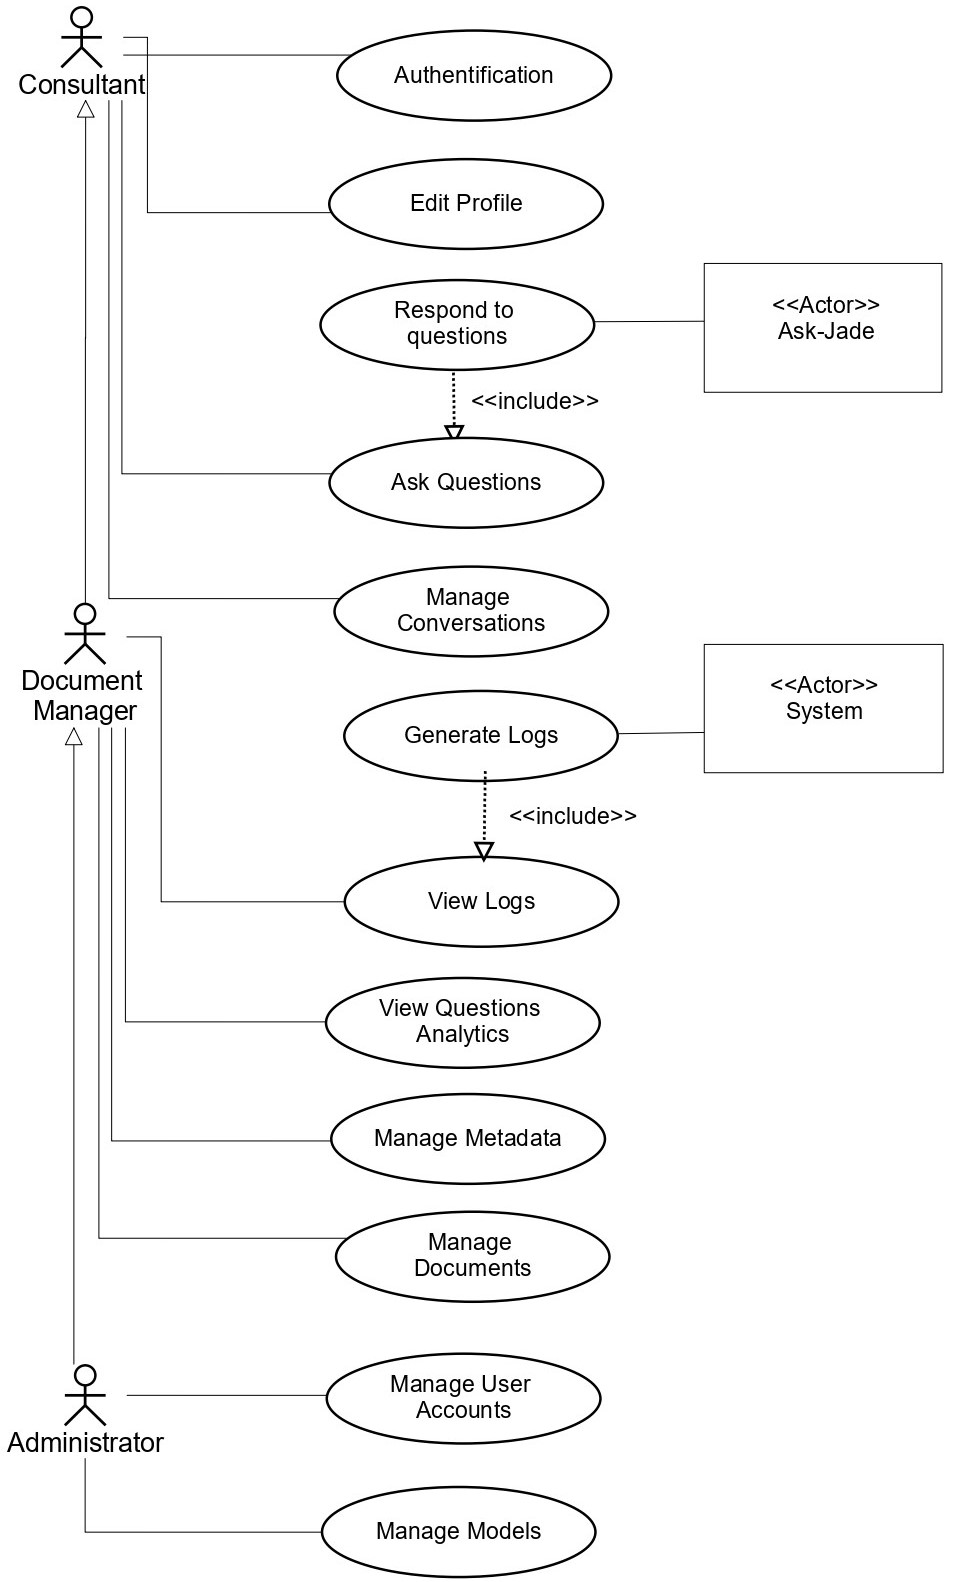
\includegraphics[width=0.9\textwidth]{ask-jade-use-case.jpg}
    \caption{Use Case Diagram}
\end{figure}


\subsection{Use Case Refinement}

The following subsections present the detailed refinement of the main use cases identified in the system, describing the actors, scenarios, preconditions, postconditions, and possible exceptions associated with each functionality.

\subsubsection{a- Manage Users}

This figure presents the use case diagram of Manage Users:

\begin{figure}[H]
    \centering
     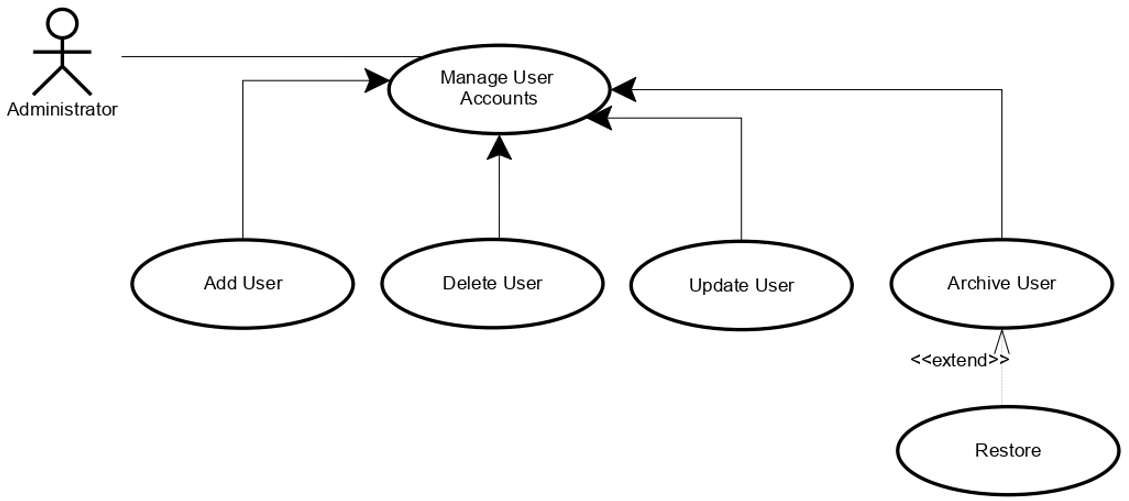
\includegraphics[width=\textwidth]{Manage Users.png}
    \caption{Use Case Diagram of Manage Users}
\end{figure}

\begin{table}[H]
\centering
\caption{Refinement of the Use Case Manage Users}
\begin{tabular}{|>{\centering\arraybackslash}p{4cm}|p{10cm}|}
\hline
\textbf{Use Case} & Manage Users \\ \hline
\textbf{Actor} & Administrator \\ \hline
\textbf{Precondition} & System is running, administrator is authenticated. \\ \hline
\textbf{Postcondition} & Users are successfully managed (created, updated, archived, restored, or deleted). \\ \hline
\textbf{Main Scenario} &
The administrator accesses the Users section. The system displays the list of registered users with their roles, status, and creation date. \\ \hline
\textbf{Alternative Scenarios} &
\parbox[t]{10cm}{\small\setlength{\parskip}{1pt}
The administrator searches or filters users by name, email, or role.\newline
The administrator selects \textbf{Add User}:\newline
\hspace*{0.2cm}-- The system displays the invitation form.\newline
\hspace*{0.2cm}-- The administrator fills in the required fields and confirms.\newline
\hspace*{0.2cm}-- The system sends an activation email and marks the user as Pending.\newline
The administrator chooses to \textbf{edit} a user:\newline
\hspace*{0.2cm}-- The system displays the update form.\newline
\hspace*{0.2cm}-- The administrator modifies the profile information and confirms.\newline
The administrator chooses to \textbf{archive} a user:\newline
\hspace*{0.2cm}-- The system archives the user, who remains visible with reduced opacity.\newline
The administrator chooses to \textbf{restore} an archived user:\newline
\hspace*{0.2cm}-- The system restores the user.\newline
The administrator chooses to \textbf{delete} a user:\newline
\hspace*{0.2cm}-- The system permanently deletes the user after confirmation.\newline
The administrator triggers a \textbf{refresh} to reload the user list.
}\\ \hline
\textbf{Exception Scenario} &
\parbox[t]{10cm}{\small\setlength{\parskip}{1pt}
-- If not authenticated, the system redirects to the login page.\newline
-- If users cannot be retrieved, an error message is displayed.\newline
-- If a required field is missing, the system displays a validation error.\newline
-- If the email already exists, the user creation is rejected.
}\\ \hline
\end{tabular}
\end{table}


\subsubsection{b- Authenticate }

This figure presents the use case diagram of Authenticate User:

\begin{figure}[H]
    \centering
     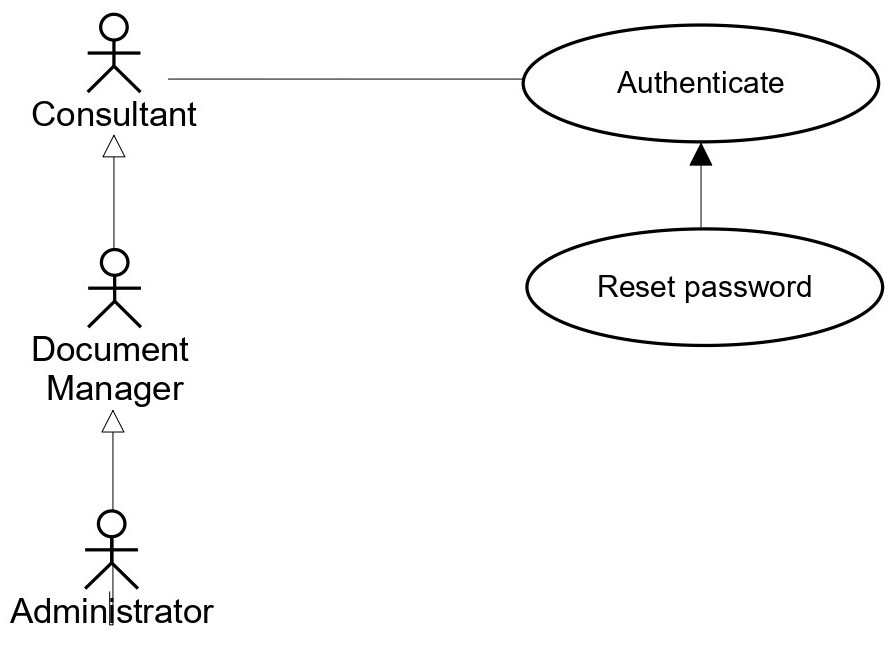
\includegraphics[width=0.55\textwidth]{authenticate.jpg}
    \caption{Use Case Diagram of Authenticate}
\end{figure}


\begin{table}[H]
\centering
\caption{Refinement of the Use Case Authenticate}
\begin{tabular}{|>{\centering\arraybackslash}p{4cm}|p{10cm}|}
\hline

\textbf{Use Case} & Authenticate \\ \hline
\textbf{Actor} & Administrator, Consultant, Document Manager \\ \hline
\textbf{Precondition} & System is running. \\ \hline
\textbf{Postcondition} & User is successfully authenticated and redirected to the dashboard. \\ \hline

\textbf{Main Scenario} &
The system displays the authentication interface. \\ \hline

\textbf{Alternative Scenarios} &
\parbox[t]{10cm}{\small\setlength{\parskip}{1pt}
The user enters their credentials and optionally activates \textbf{Remember Me}.\newline
The user selects \textbf{Sign In}:\newline
\hspace*{0.2cm}-- The system verifies the credentials and redirects to the dashboard.\newline
The user selects \textbf{Forgot your password?}:\newline
\hspace*{0.2cm}-- The user submits their email address.\newline
\hspace*{0.2cm}-- The system sends a password reset link by email.\newline
The user follows the reset link:\newline
\hspace*{0.2cm}-- The user enters and confirms the new password.\newline
\hspace*{0.2cm}-- The system updates the password and redirects to the sign in page.
}\\ \hline

\textbf{Exception Scenario} &
\parbox[t]{10cm}{\small\setlength{\parskip}{1pt}
-- If credentials are incorrect, an error message is displayed.\newline
-- If the account is locked after multiple failed attempts, a temporary lock message is displayed.\newline
-- If passwords do not match during reset, an error message is displayed.
}\\ \hline

\end{tabular}
\end{table}

\subsubsection{c- Edit Profile}

This figure presents the use case diagram of Edit Profile:

\begin{figure}[H]
    \centering
     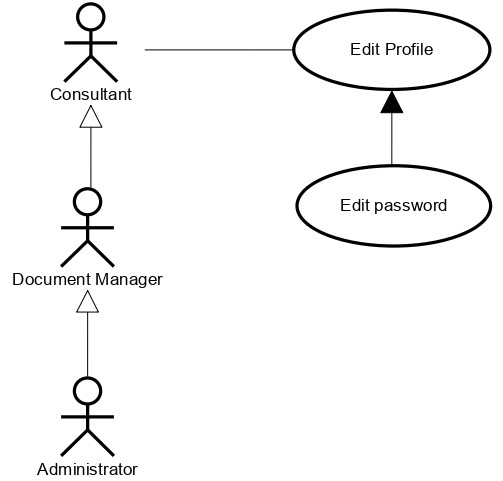
\includegraphics[width=0.55\textwidth]{Edit profile.jpg}
    \caption{Use Case Diagram of Edit profile}
\end{figure}

\begin{table}[H]
\centering
\caption{Refinement of the Use Case Edit Profile}
\begin{tabular}{|>{\centering\arraybackslash}p{4cm}|p{10cm}|}
\hline

\textbf{Use Case} & Edit Profile \\ \hline
\textbf{Actor} & Administrator, Consultant, Document Manager \\ \hline
\textbf{Precondition} & User is authenticated and connected to the system. \\ \hline
\textbf{Postcondition} & User profile or password is successfully updated. \\ \hline

\textbf{Main Scenario} &
The user accesses the profile menu from the header. The system displays a dropdown with available options. \\ \hline

\textbf{Alternative Scenarios} &
\parbox[t]{10cm}{\small\setlength{\parskip}{1pt}
The user selects \textbf{Edit Profile}:\newline
\hspace*{0.2cm}-- The user updates the required fields and confirms.\newline
\hspace*{0.2cm}-- The system validates and saves the profile successfully.\newline
The user selects \textbf{Edit Password}:\newline
\hspace*{0.2cm}-- The user enters the current password, then the new password and its confirmation.\newline
\hspace*{0.2cm}-- The system verifies and updates the password successfully.
}\\ \hline

\textbf{Exception Scenario} &
\parbox[t]{10cm}{\small\setlength{\parskip}{1pt}
-- If required fields are empty, a validation error is displayed.\newline
-- If the current password is incorrect, an error message is displayed.\newline
-- If the new password and confirmation do not match, an error message is displayed.\newline
-- If a server error occurs, an error message is displayed.
}\\ \hline

\end{tabular}
\end{table}





\subsubsection{d- Ask Questions}

This figure presents the use case diagram of Ask Questions:

\begin{figure}[H]
    \centering
     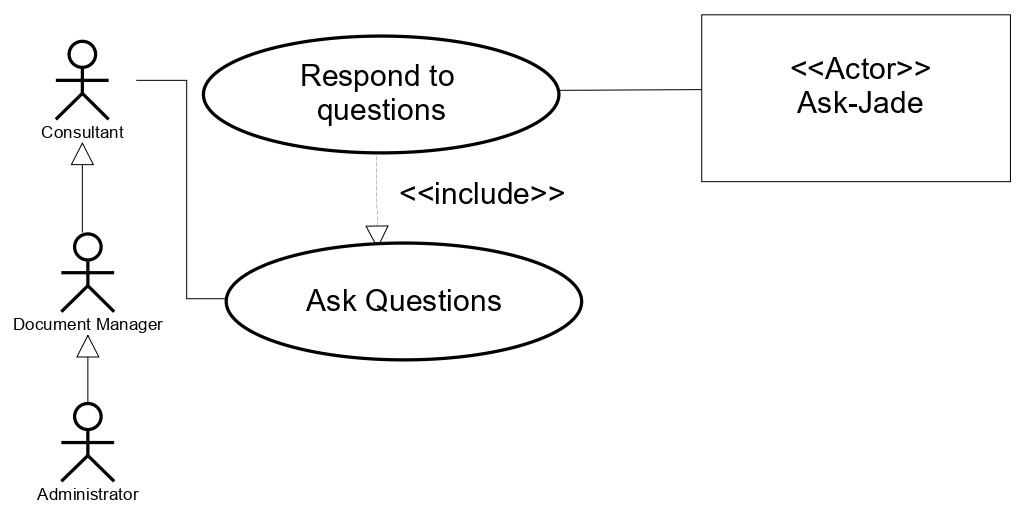
\includegraphics[width=0.8\textwidth]{ask questions.jpg}
    \caption{Use Case Diagram of Ask Questions}
\end{figure}

\begin{table}[H]
\centering
\caption{Refinement of the Use Case Ask Questions}
\begin{tabular}{|>{\centering\arraybackslash}p{4cm}|p{10cm}|}
\hline

\textbf{Use Case} & Ask Questions \\ \hline
\textbf{Actor} & Administrator, Consultant, Document Manager \\ \hline
\textbf{Precondition} & User is authenticated and has access to the chat interface. \\ \hline
\textbf{Postcondition} & The system provides an answer to the user's question. \\ \hline

\textbf{Main Scenario} &
The system displays the chat interface. \\ \hline

\textbf{Alternative Scenarios} &
\parbox[t]{10cm}{\small\setlength{\parskip}{1pt}
The user enters a question and submits it:\newline
\hspace*{0.2cm}-- The system processes the request and displays the generated response.\newline
\hspace*{0.2cm}-- The system displays sources related to the answer.
}\\ \hline

\textbf{Exception Scenario} &
\parbox[t]{10cm}{\small\setlength{\parskip}{1pt}
-- If the message is empty, the request is not submitted.\newline
-- If an error occurs, an error message is displayed.
}\\ \hline

\end{tabular}
\end{table}




\subsubsection{e- Manage Conversations}

This figure presents the use case diagram of Manage Conversations:

\begin{figure}[H]
    \centering
     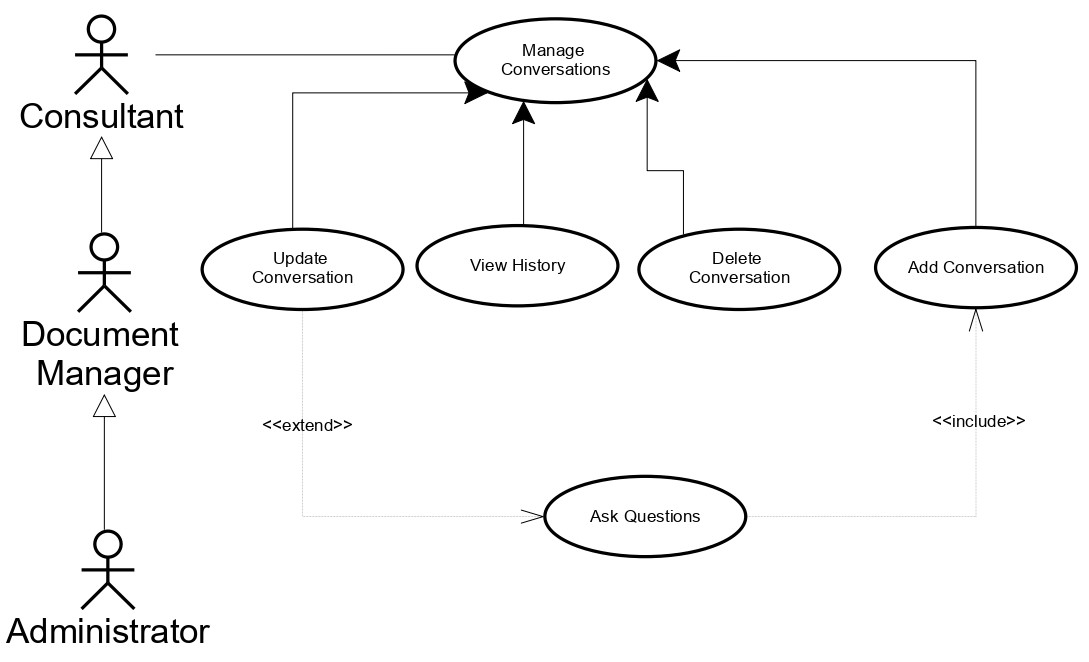
\includegraphics[width=\textwidth]{Manage Conversation.jpg}
    \caption{Use Case Diagram of Manage Conversations}
\end{figure}

\begin{table}[H]
\centering
\caption{Refinement of the Use Case Manage Conversations}
\begin{tabular}{|>{\centering\arraybackslash}p{4cm}|p{10cm}|}
\hline

\textbf{Use Case} & Manage Conversations \\ \hline
\textbf{Actor} & Administrator, Consultant, Document Manager \\ \hline
\textbf{Precondition} & User is authenticated. \\ \hline
\textbf{Postcondition} & Conversations are created, viewed, updated, or deleted successfully. \\ \hline

\textbf{Main Scenario} &
The system displays the list of conversations. \\ \hline

\textbf{Alternative Scenarios} &
\parbox[t]{10cm}{\small\setlength{\parskip}{1pt}
The user initiates a \textbf{New Conversation}:\newline
\hspace*{0.2cm}-- The system creates and adds it to the list.\newline
The user selects a \textbf{conversation} to view its content.\newline
The user searches for a conversation by title or preview.\newline
The user chooses to \textbf{edit} a conversation title:\newline
\hspace*{0.2cm}-- The user modifies the title and the system saves it.\newline
The user chooses to \textbf{delete} a conversation:\newline
\hspace*{0.2cm}-- The system requests confirmation before deletion.
}\\ \hline

\textbf{Exception Scenario} &
\parbox[t]{10cm}{\small\setlength{\parskip}{1pt}
-- If no conversation exists, an empty state is displayed.\newline
-- If an error occurs while loading, an error message is displayed.
}\\ \hline

\end{tabular}
\end{table}





\subsubsection{f- Manage Documents}

This figure presents the use case diagram of Manage Documents:

\begin{figure}[H]
    \centering
    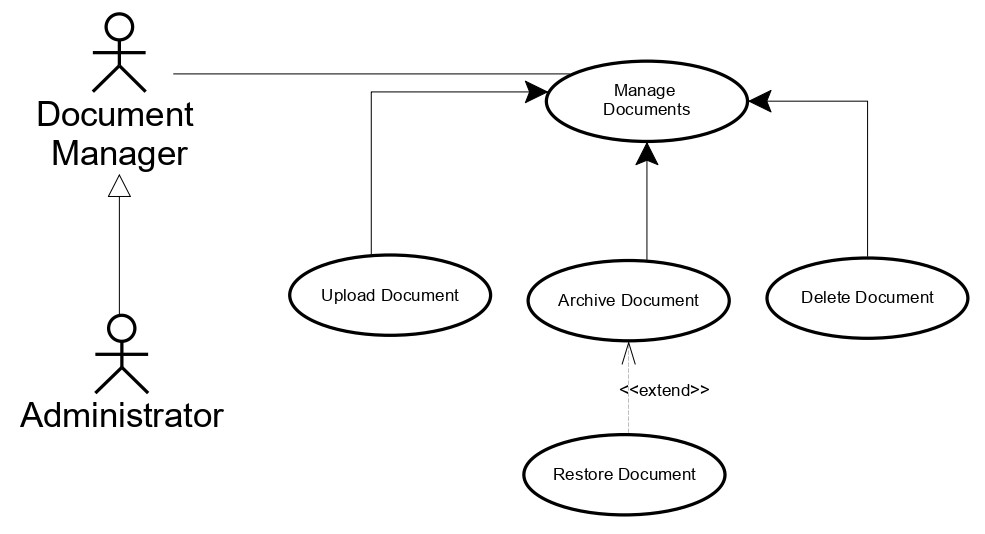
\includegraphics[width=\textwidth]{Manage Documents.jpg}
    \caption{Use Case Diagram of Manage Documents}
\end{figure}

\begin{table}[H]
\centering
\caption{Refinement of the Use Case Manage Documents}
\begin{tabular}{|>{\centering\arraybackslash}p{4cm}|p{10cm}|}
\hline

\textbf{Use Case} & Manage Documents \\ \hline
\textbf{Actor} & Administrator, Document Manager \\ \hline
\textbf{Precondition} & User is authenticated. \\ \hline
\textbf{Postcondition} & Documents are uploaded, archived, restored, or deleted successfully. \\ \hline

\textbf{Main Scenario} &
The system displays the list of documents. \\ \hline

\textbf{Alternative Scenarios} &
\parbox[t]{10cm}{\small\setlength{\parskip}{1pt}
The user initiates an \textbf{Upload Document}:\newline
\hspace*{0.2cm}-- The system processes the file and adds it to the list.\newline
The user chooses to \textbf{archive} a document:\newline
\hspace*{0.2cm}-- The system archives the selected document.\newline
The user chooses to \textbf{restore} an archived document:\newline
\hspace*{0.2cm}-- The system restores it.\newline
The user chooses to \textbf{delete} a document:\newline
\hspace*{0.2cm}-- The system requests confirmation before deletion.
}\\ \hline

\textbf{Exception Scenario} &
\parbox[t]{10cm}{\small\setlength{\parskip}{1pt}
-- If no document exists, an empty state is displayed.\newline
-- If an error occurs during upload or processing, an error message is displayed.\newline
-- If deletion fails, the user is notified.
}\\ \hline

\end{tabular}
\end{table}




\subsubsection{g- Manage Metadata}

This figure presents the use case diagram of Manage Metadata:

\begin{figure}[H]
    \centering
    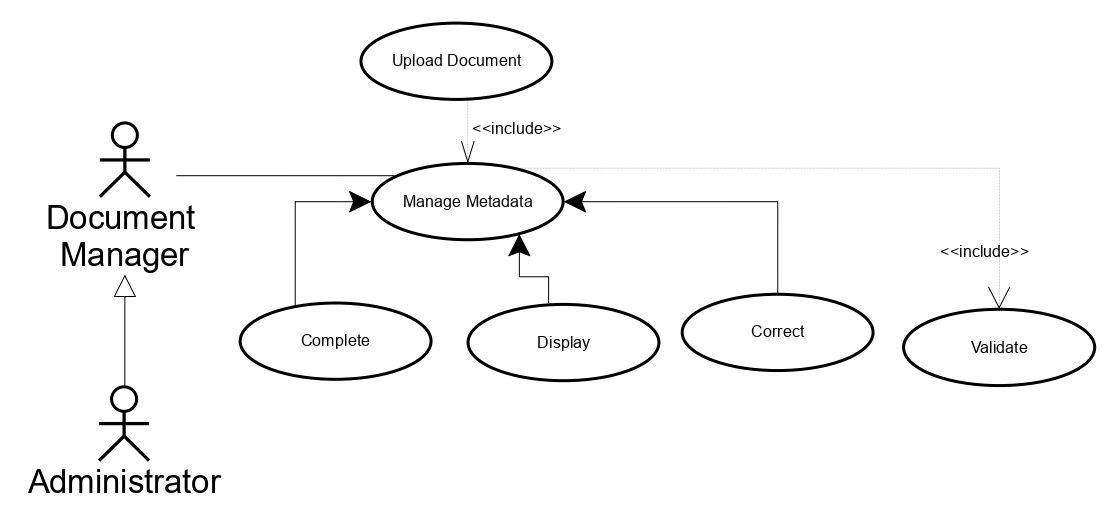
\includegraphics[width=\textwidth]{Manage Metadata.jpg}
    \caption{Use Case Diagram of Manage Metadata}
\end{figure}

\begin{table}[H]
\centering
\caption{Refinement of the Use Case Manage Metadata}
\begin{tabular}{|>{\centering\arraybackslash}p{4cm}|p{10cm}|}
\hline

\textbf{Use Case} & Manage Metadata \\ \hline
\textbf{Actor} & Administrator, Document Manager \\ \hline
\textbf{Precondition} & Document is uploaded and processed. \\ \hline
\textbf{Postcondition} & Metadata is completed, corrected, and validated successfully. \\ \hline

\textbf{Main Scenario} &
The system displays the extracted metadata of the document. \\ \hline

\textbf{Alternative Scenarios} &
\parbox[t]{10cm}{\small\setlength{\parskip}{1pt}
The system automatically extracts metadata after upload.\newline
The user completes any missing fields such as author, type, or language.\newline
The user chooses to \textbf{correct} metadata:\newline
\hspace*{0.2cm}-- The user modifies incorrect fields and the system updates them.\newline
The user chooses to \textbf{validate} metadata:\newline
\hspace*{0.2cm}-- The user selects a project and the system saves the metadata.
}\\ \hline

\textbf{Exception Scenario} &
\parbox[t]{10cm}{\small\setlength{\parskip}{1pt}
-- If extraction fails, manual input is allowed.\newline
-- If required fields are missing, validation is prevented.\newline
-- If an error occurs during validation, an error message is displayed.
}\\ \hline

\end{tabular}
\end{table}




\subsubsection{h- View Logs}

This figure presents the use case diagram of View Logs:

\begin{figure}[H]
    \centering
    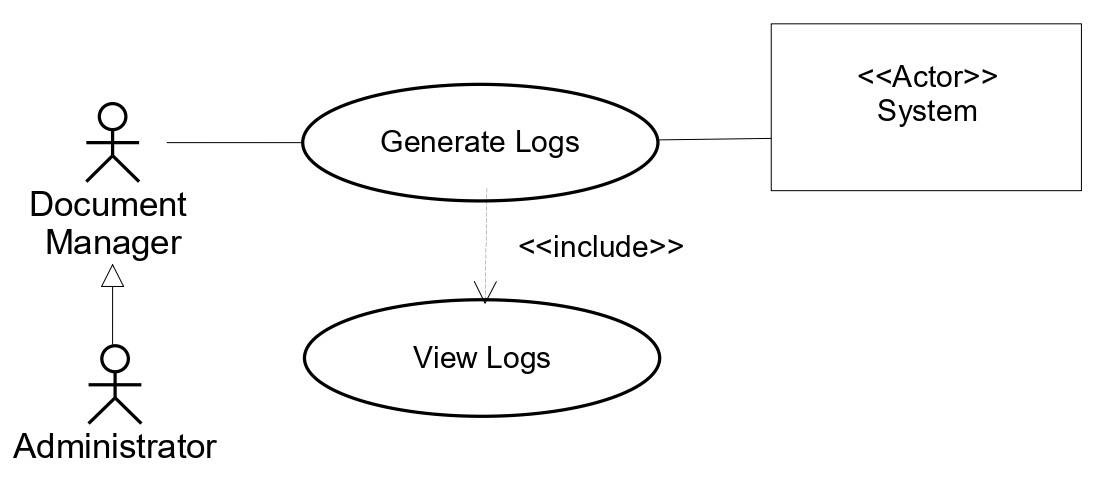
\includegraphics[width=0.6\textwidth]{view logs.jpg}
    \caption{Use Case Diagram of View Logs}
\end{figure}

\begin{table}[H]
\centering
\caption{Refinement of the Use Case View Logs}
\begin{tabular}{|>{\centering\arraybackslash}p{4cm}|p{10cm}|}
\hline

\textbf{Use Case} & View Logs \\ \hline
\textbf{Actor} & Administrator, Document Manager \\ \hline
\textbf{Precondition} & User is authenticated and has access to audit logs. \\ \hline
\textbf{Postcondition} & Logs are displayed, filtered, and optionally exported. \\ \hline

\textbf{Main Scenario} &
The system displays the list of audit logs. \\ \hline

\textbf{Alternative Scenarios} &
\parbox[t]{10cm}{\small\setlength{\parskip}{1pt}
The user filters logs by category (documents, users, system, security).\newline
The user browses the logs list to view details such as action, user, timestamp, and description.\newline
The user initiates an \textbf{Export Logs}:\newline
\hspace*{0.2cm}-- The system generates and downloads the log file.\newline
The system automatically records each user or system action as a log entry.
}\\ \hline

\textbf{Exception Scenario} &
\parbox[t]{10cm}{\small\setlength{\parskip}{1pt}
-- If no logs exist, an empty state is displayed.\newline
-- If an error occurs while loading, an error message is displayed.\newline
-- If export fails, the user is notified.
}\\ \hline

\end{tabular}
\end{table}

\subsubsection{i- View Analytics}

This figure presents the use case diagram of View Analytics:

\begin{figure}[H]
    \centering
    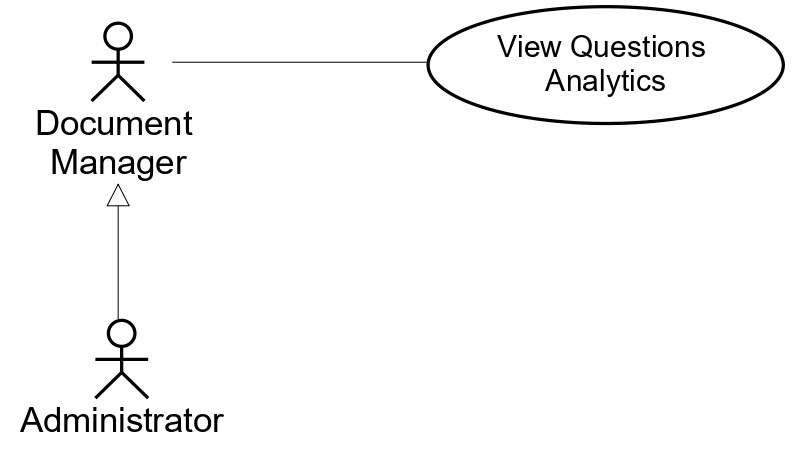
\includegraphics[width=0.6\textwidth]{view analytics questions.jpg}
    \caption{Use Case Diagram of View Analytics}
\end{figure}

\begin{table}[H]
\centering
\caption{Refinement of the Use Case View Analytics}
\begin{tabular}{|>{\centering\arraybackslash}p{4cm}|p{10cm}|}
\hline

\textbf{Use Case} & View Analytics \\ \hline
\textbf{Actor} & Administrator \\ \hline
\textbf{Precondition} & User is authenticated and has admin privileges. \\ \hline
\textbf{Postcondition} & Analytics data is displayed and interpreted successfully. \\ \hline

\textbf{Main Scenario} &
The system displays analytics dashboards including system performance and usage metrics. \\ \hline

\textbf{Alternative Scenarios} &
\parbox[t]{10cm}{\small\setlength{\parskip}{1pt}
The system displays \textbf{system performance metrics} such as response time, uptime, and health indicators.\newline
The system displays \textbf{model performance} including response accuracy and number of processed queries.\newline
The system displays \textbf{most asked questions} and \textbf{usage statistics} such as active users and interactions.\newline
The system displays \textbf{user feedback} including ratings and comments on system responses.\newline
The user initiates an \textbf{Export Report}:\newline
\hspace*{0.2cm}-- The system generates and downloads the analytics report.
}\\ \hline

\textbf{Exception Scenario} &
\parbox[t]{10cm}{\small\setlength{\parskip}{1pt}
-- If no analytics data is available, an empty state is displayed.\newline
-- If an error occurs while loading, an error message is displayed.\newline
-- If charts fail to load, placeholders are displayed.
}\\ \hline

\end{tabular}
\end{table}


\section{Conceptual Study}

This section presents the architectural and dynamic views of the Ask-Jade
system through deployment, activity, and sequence diagrams.


\subsection{Deployment Diagram}
Figure \textbf{3.11} illustrates the physical deployment architecture
of Ask-Jade.

\begin{figure}[H]
  \centering
  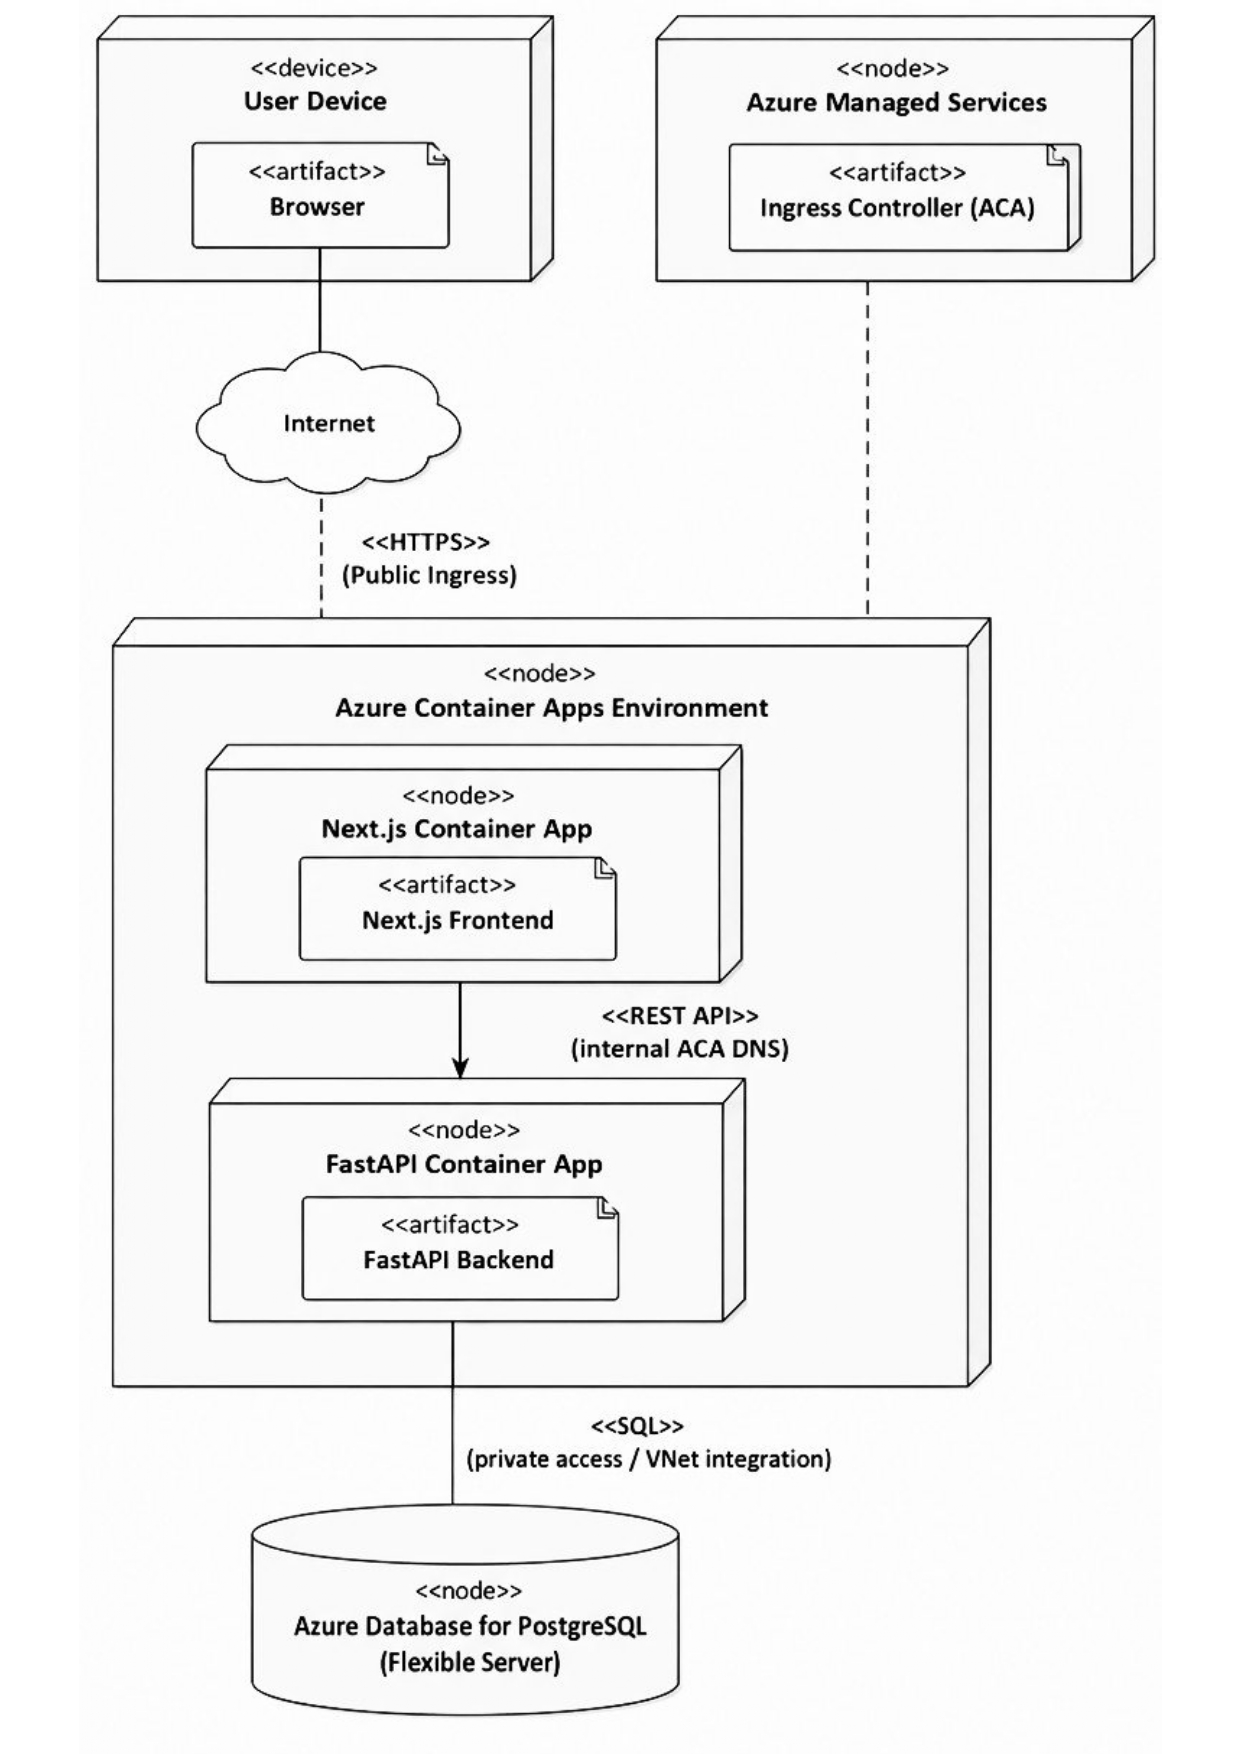
\includegraphics[width=0.9\textwidth]{dep.jpg}
  \caption{Deployment Diagram of the Ask-Jade System}
  \label{fig:deployment}
\end{figure}




\subsection{Ask Question Activity Diagram}

Figure \textbf{3.12} illustrates the activity flow of the RAG pipeline,
from query processing and retrieval to answer generation.

\begin{figure}[H]
\centering
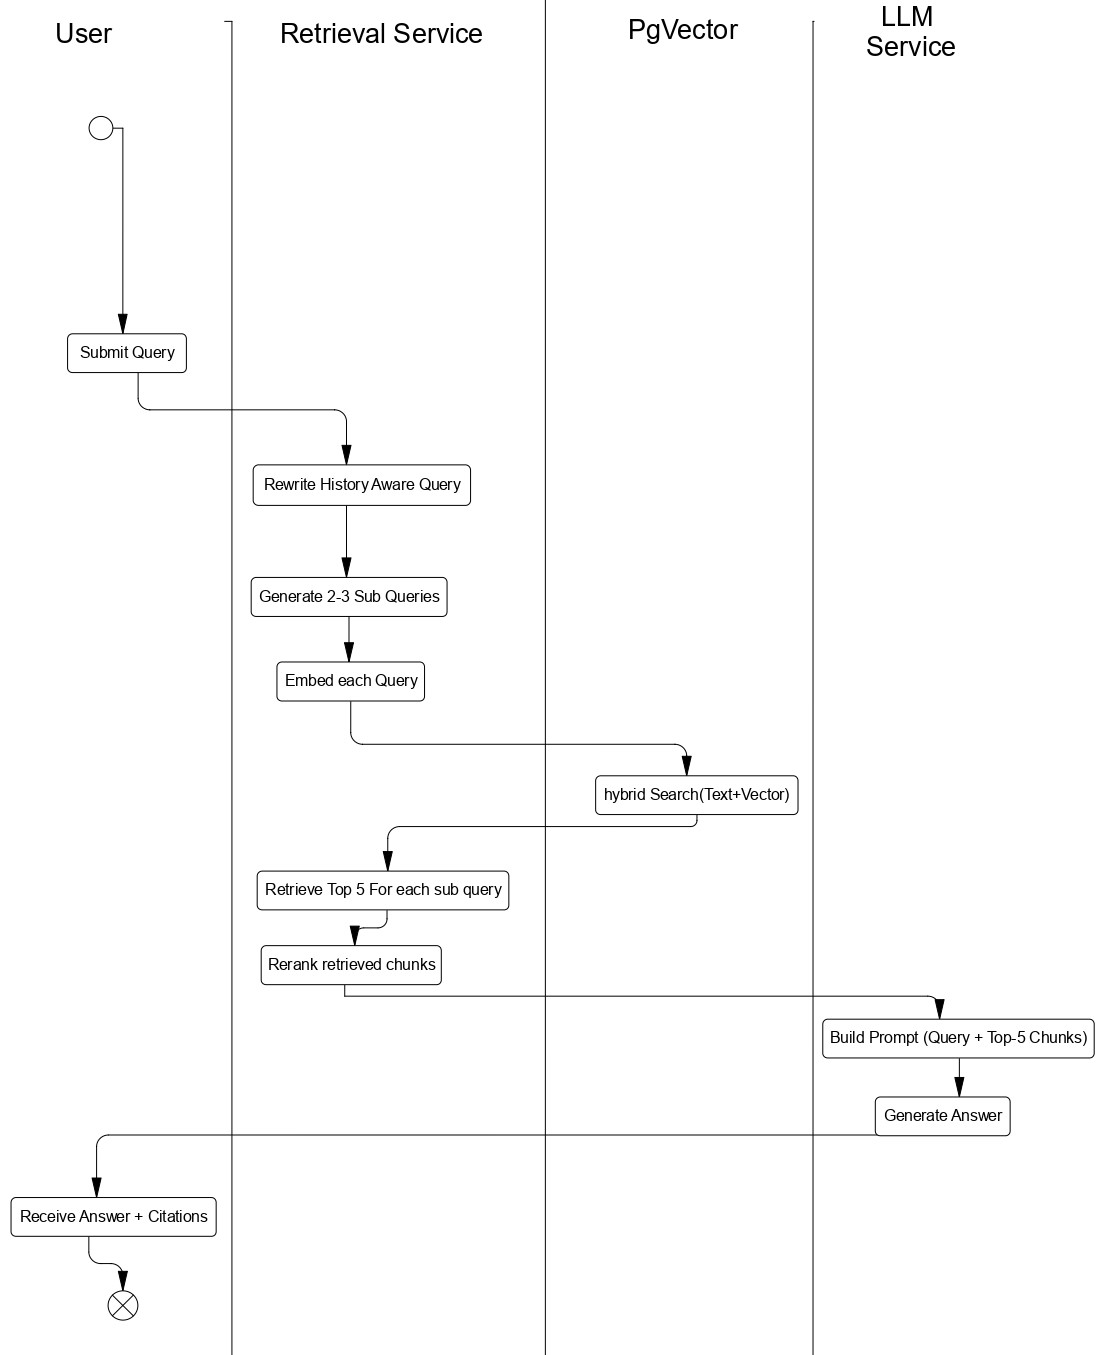
\includegraphics[width=\textwidth]{activity_ask_question.jpg}
\caption{Activity Diagram for the Ask Question Use Case}
\label{fig:activity_ask_question}
\end{figure}



\begin{figure}[H]
    \centering
    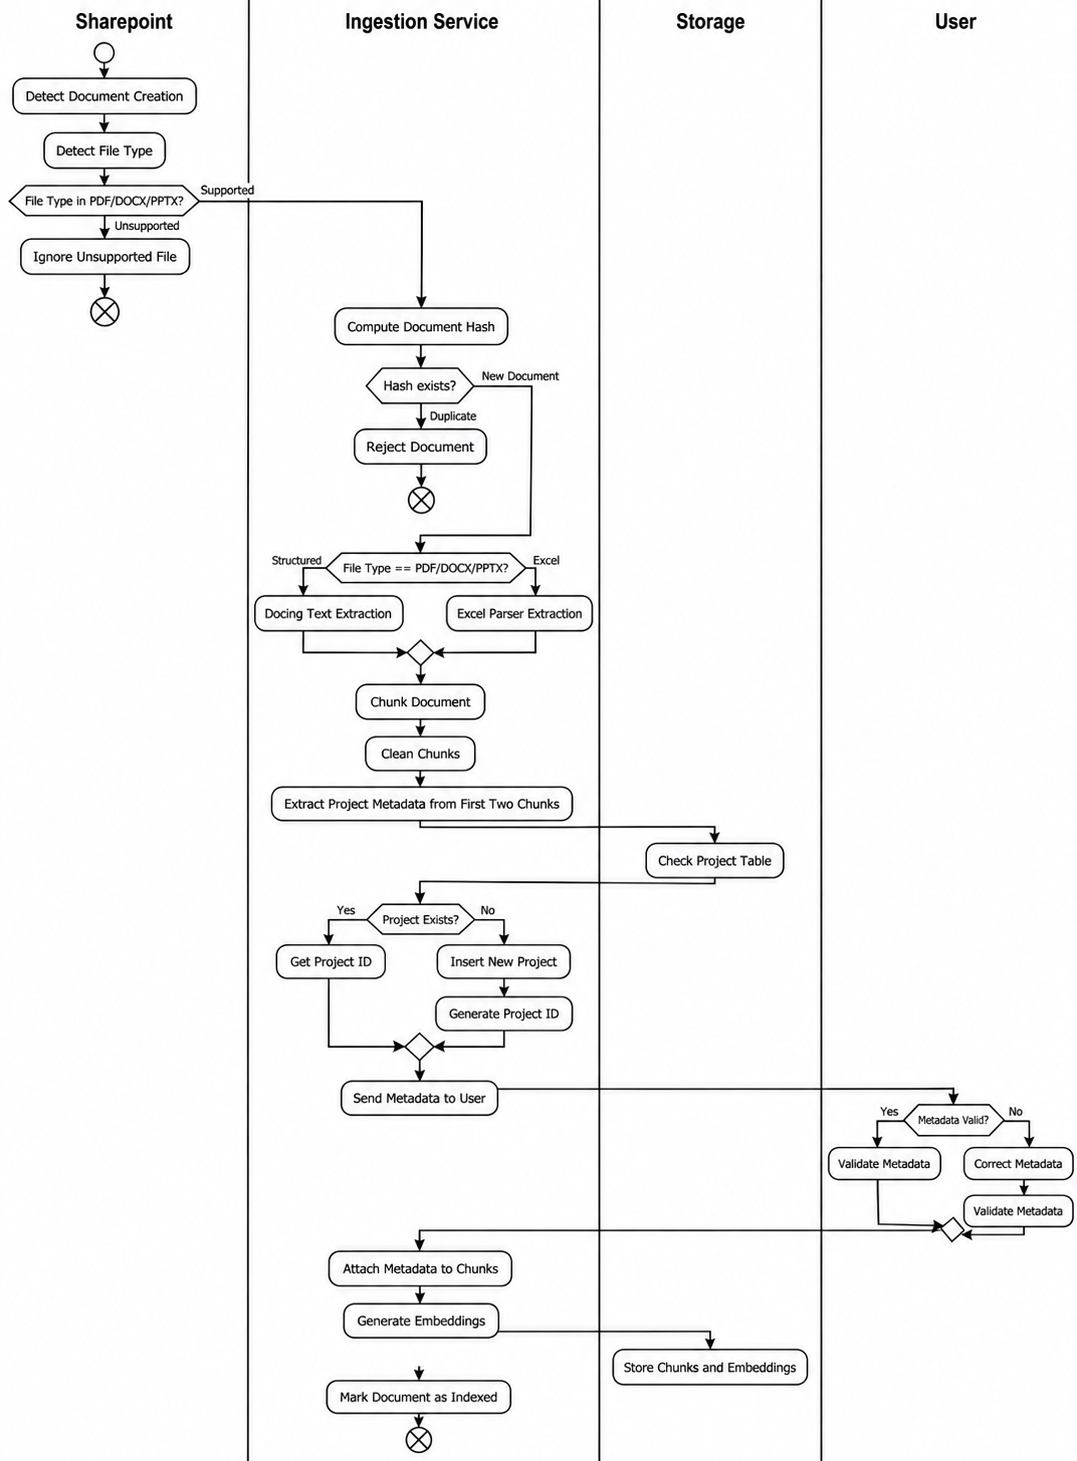
\includegraphics[width=\textwidth]{activity_document.png}
    \caption{Sequence Diagram for Manage Documents Use Case}
    \label{fig:seq_manage_documents}
\end{figure}








